\documentclass[12pt, a4paper, twoside]{article}

%% Preamble
\usepackage{pdfpages}           % Para incluir PDFs
\usepackage{graphicx}           % Para gráficos
\usepackage{subfiles}           % Para manejar subarchivos
\usepackage{hyperref}           % Para enlaces
\usepackage{listings}           % Para código fuente (ajusta lenguaje)
\usepackage{verbatim}
\usepackage[backend=bibtex,style=numeric]{biblatex} % Para citas numéricas
\addbibresource{references.bib} % Cargar archivo .bib
\usepackage{url}
\usepackage{float}


\usepackage{geometry}           % Para ajustar márgenes

% Ajustes de márgenes
\geometry{
	left=3cm,       % Margen izquierdo
	right=3cm,      % Margen derecho
	top=2.5cm,      % Margen superior
	bottom=2.5cm,   % Margen inferior
	headheight=15pt, % Altura del encabezado
	twoside          % Para documentos a dos caras
}


\graphicspath{{images/}{../images/}} % Ruta para imágenes

\begin{document}
	
	%% Cover
	
\includepdf[noautoscale=true, width=\paperwidth]{cover.pdf}
	
	%% Title
	\clearpage
	\setcounter{page}{1}
	
\includepdf[noautoscale=true, width=\paperwidth]{title.pdf}
	
	%%%%%%%%%%%%%%%%%%%%%%%%%%%%%%%%%%%%%%%%%%%%%%%%%%%%%%%%%%%%%%%%%%%%%%%%%%%
	
	% Índice automático
	\tableofcontents
	\newpage
	
	\section{Introducción}
	
	Este documento constituye una continuación del trabajo previo, donde se desarrolló el diseño conceptual y lógico de un almacén de datos basado en la información proporcionada por la \textit{Base de Datos de Investigación Colaborativa eICU} \cite{eICU2024}. En ese proyecto, el enfoque principal fue la selección y análisis de información relativa a \textbf{pacientes con patologías respiratorias}, determinando las tablas y columnas más relevantes para permitir un análisis exhaustivo de esta población específica.
	
	En esta nueva fase, se procederá a la implementación del proceso de \textbf{Extracción, Transformación y Carga} (ETL, por sus siglas en inglés). Este proceso es fundamental para la integración de datos en cualquier almacén de datos, ya que permite extraer datos de múltiples fuentes, transformarlos según las necesidades del modelo, y finalmente cargarlos en el sistema de almacenamiento. El proceso ETL es clave para garantizar la calidad, consistencia e integridad de los datos, factores esenciales para que el análisis posterior sea preciso y confiable.
	
	El éxito de este proceso asegura que las tablas del almacén de datos estén adecuadamente pobladas con información precisa, sentando las bases para un \textbf{análisis de datos} eficiente. Este proceso facilita la realización de consultas complejas o la integración de herramientas como \textit{Reporting Services}, que permiten la visualización clara y sencilla de la información más relevante, apoyando la toma de decisiones clínicas fundamentadas.
	
	Por lo tanto, este documento también incluirá un tutorial detallado del proceso de carga para las tablas del almacén de datos personalizado. Además, se presentará un análisis de las dificultades encontradas durante la implementación y las estrategias empleadas para superarlas.
	
	\section{Objetivos}
	
	El principal objetivo de este informe es documentar de manera detallada la ejecución del proceso ETL en dos contextos diferentes:
	
	\begin{itemize}
		\item El almacén de datos \textit{NorthwindDW}, utilizado como referencia durante las sesiones prácticas, cuya carga será replicada siguiendo los procedimientos previamente establecidos.
		\item El almacén de datos del \textit{eICU}, adaptado específicamente para el análisis de \textbf{pacientes con patologías respiratorias}, que será implementado utilizando el modelo lógico desarrollado en la fase anterior del proyecto.
	\end{itemize}
	
	A lo largo del documento se mostrará cómo se ha llevado a cabo la integración de datos en ambos almacenes, resaltando los desafíos enfrentados y las soluciones aplicadas, con el fin de proporcionar una guía clara y replicable del proceso.
	
	 
	
	\section{Modificación del almacén de datos}
	
	Durante la implementación del almacén de datos se realizaron diversas modificaciones en su estructura original, con el fin de adaptarlo lo mejor posible siguiendo las mejores prácticas para crear un buen almacén de datos. A continuación, se detallan los principales cambios efectuados y la justificación detrás de cada uno de ellos (puede ver también la figura \ref{fig:1}).
	
	
	\begin{figure}[h!]
		\centering
		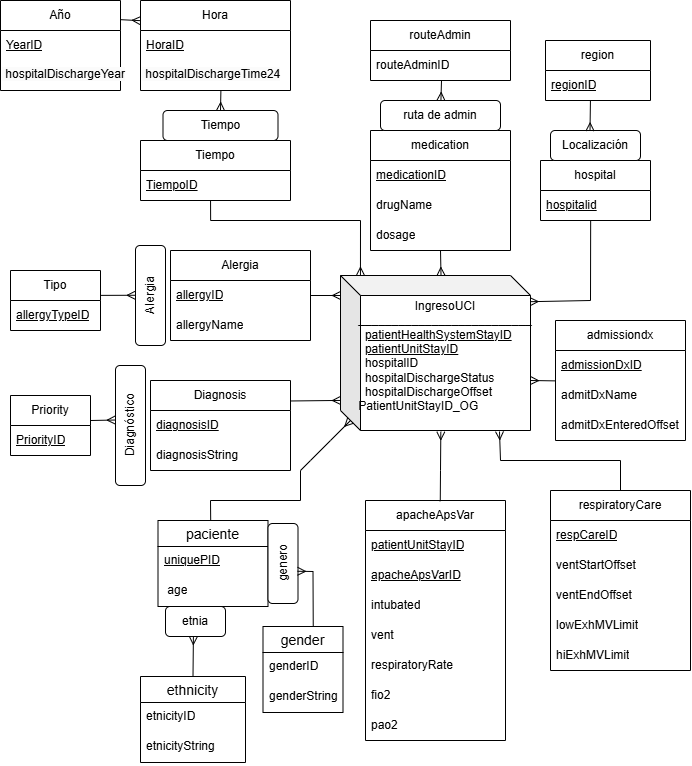
\includegraphics[width=1\textwidth]{image/diagrama_correcicones.png}
		\caption{Diagrama actualizado (Correcciones implementadas)}
		\label{fig:1}
	\end{figure}
	
	\subsection{Ingreso a la UCI}
	El mayor cambio que hubo es que el hecho Ingreso a la UCI fue separado de la tabla paciente, Además se incorporó el atributo \texttt{hospitalDischargeOffset}, que indica la duración de la estancia del paciente en la UCI, medida en minutos desde el ingreso hasta el alta hospitalaria. Este ajuste fue sugerido para permitir el análisis del tiempo de hospitalización de cada paciente, un factor relevante en los estudios de recuperación y tratamiento de enfermedades respiratorias.
	
	\subsection{Tiempo de Alta}
	Para estudiar el tiempo en este proyecto se decidió almacenar únicamente los atributos \texttt{hospitalDischargeTime24} y \texttt{hospitalDischargeYear}, ya que la base de datos no contiene un campo \texttt{hospitalAdmitYear}, como se había sugerido originalmente. Esta decisión se tomó con base en la disponibilidad de datos y la coherencia con el diseño del modelo lógico.
	
	\subsection{Paciente}
	La tabla \textbf{Paciente}, cuyo identificador único (\texttt{PK}) es el campo \texttt{uniquePID}. Además de este identificador, se incluyeron atributos relevantes como la \texttt{edad}. También se estableció una jerarquía paralela para \textbf{género} y \textbf{etnia}, lo que permitió organizar estos atributos de forma más estructurada y lógica.
	
	\subsection{Supresión de Respiratory Charting}
	La tabla \textbf{Respiratory Charting}, fue eliminada al trabajar más detenidamente en ella se observó múltiples inconsistencias como es la baja cantidad de datos en comparación a otros datos, cierto parentesco para algunas métricas que ya se calculaban en \textit{ApacheApsVar} y que dependiendo del paciente se le hacía una métrica especifica, lo cual terminaba siendo rellenado con cierta cantidad de errores. En búsqueda de mantener un almacén más claro y simple se elimina esta tabla del DDL.
	
	\subsection{Almacenamiento del identificador del paciente de la base de datos original}
	
	El proceso ETL es complejo y puede generar dependencias para mantener la coherencia de las relaciones entre las tablas. En el caso de los datos de eICU, existen múltiples tablas con relaciones de tipo M:N con el hecho principal, lo que requiere la creación de tablas intermedias en el almacén de datos. Para establecer estas relaciones, es necesario incluir un atributo que vincule las tablas de forma adecuada. Por esta razón, se creó el atributo \textit{PatientUnitStayID\_OG}, que almacena el identificador del paciente original de la base de datos eICU. Este identificador es esencial, ya que al migrar los datos al nuevo almacén, se utilizará para vincular las nuevas claves autogeneradas. 
	
	Un ejemplo de este proceso es la tabla de alergias, que, además de almacenar el nombre de la alergia y si está relacionada con un fármaco, incluye el identificador de los ingresos asociados a dicha alergia. Esto es necesario porque, en este proyecto, las claves originales fueron reemplazadas por valores autogenerados.
	
	
	\subsection{Relaciones entre Tablas}
	A continuación se describen las relaciones establecidas entre las tablas del almacén de datos, modificadas para garantizar un diseño coherente y funcional:
	
	\begin{enumerate}
		\item \textbf{Paciente} \\
		\textit{Relación: 1-n} \\
		Cada paciente puede tener múltiples ingresos a la UCI, lo que refleja que un mismo paciente puede ser readmitido en distintos momentos debido a recaídas o nuevas patologías.
		
		\item \textbf{Diagnosis} \\
		\textit{Relación: n-m} \\
		Un paciente puede tener múltiples diagnósticos asociados a un único ingreso, y el mismo diagnóstico puede repetirse en diferentes ingresos y entre distintos pacientes.
		
		\item \textbf{Medicamentos} \\
		\textit{Relación: n-m} \\
		Un ingreso puede estar asociado a la administración de varios medicamentos. Además, un medicamento puede ser utilizado en distintos ingresos de múltiples pacientes.
		
		\item \textbf{Alergia} \\
		\textit{Relación: n-m} \\
		Cada paciente puede tener múltiples alergias documentadas, las cuales son relevantes para su tratamiento durante cada ingreso a la UCI. Por lo tanto, una alergia puede estar relacionada con múltiples ingresos.
		
		\item \textbf{RespiratoryCare} \\
		\textit{Relación: 1-n} \\
		Similar a \textit{RespiratoryCharting}, cada ingreso puede tener múltiples intervenciones de cuidado respiratorio, como la administración de oxígeno o ventilación mecánica, asociadas a un ingreso específico.
		
		\item \textbf{apacheApsVar} \\
		\textit{Relación: 1-1} \\
		Cada ingreso a la UCI tiene una única evaluación APS asociada. Dependiendo del diseño, esta relación puede ser de uno a uno (si se almacena como un único resumen por ingreso) o de uno a muchos (si se almacena como varios componentes individuales evaluados), se decidió que la primera forma otorga más información y mayor relación con el hecho.
		
		\item \textbf{Admissiondx} \\
		\textit{Relación: 1-n} \\
		Cada ingreso tiene un diagnóstico primario de admisión, aunque pueden existir diagnósticos  más concretos que se documentan en otra tabla, como \textit{Diagnosis} que contiene información más clara y estudiada.
		
		\item \textbf{Hospital} \\
		\textit{Relación: 1-n} \\
		Cada hospital puede tener múltiples ingresos a la UCI. Los ingresos se asocian exclusivamente a un hospital, dependiendo del centro de atención en el que se encuentre la unidad.
	\end{enumerate}

	

	
	Los cambios en las relaciones entre tablas buscan optimizar el diseño del almacén de datos, adaptándolo a las necesidades específicas del análisis clínico de los pacientes con patologías respiratorias. Estas modificaciones garantizan la integridad de los datos y la flexibilidad para realizar análisis detallados en contextos hospitalarios. 
	
	
	\section{ETL del almacén de datos NorthwindDW}
	
	Sección de muestre la imagen de la carga completa de NorthwindDW, con todos los "ticks" en verde. 
	
	\begin{figure}[H]
		\centering
		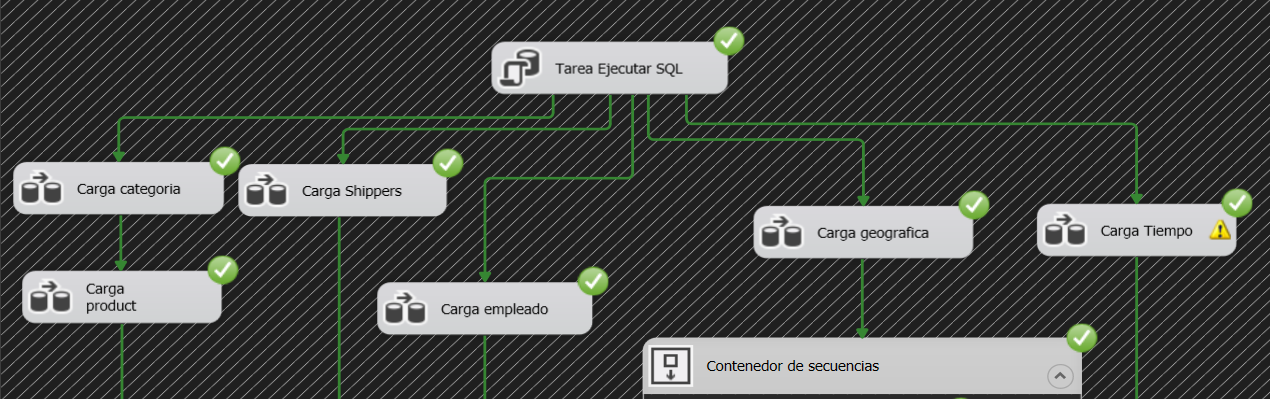
\includegraphics[width=1\textwidth]{image/flujo_north_1.png}
		\caption{Flujo ETL Nortwind PT1}
		\label{fig:5}
	\end{figure}
	
	\begin{figure}[H]
		\centering
		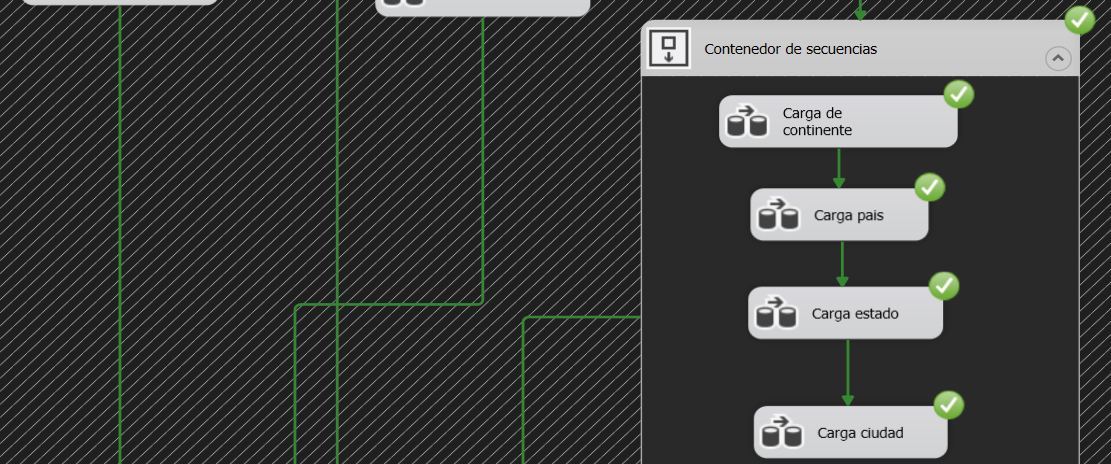
\includegraphics[width=1\textwidth]{image/flujo_north_2.png}
		\caption{Flujo ETL Nortwind PT2}
		\label{fig:6}
	\end{figure}
	
	\begin{figure}[H]
		\centering
		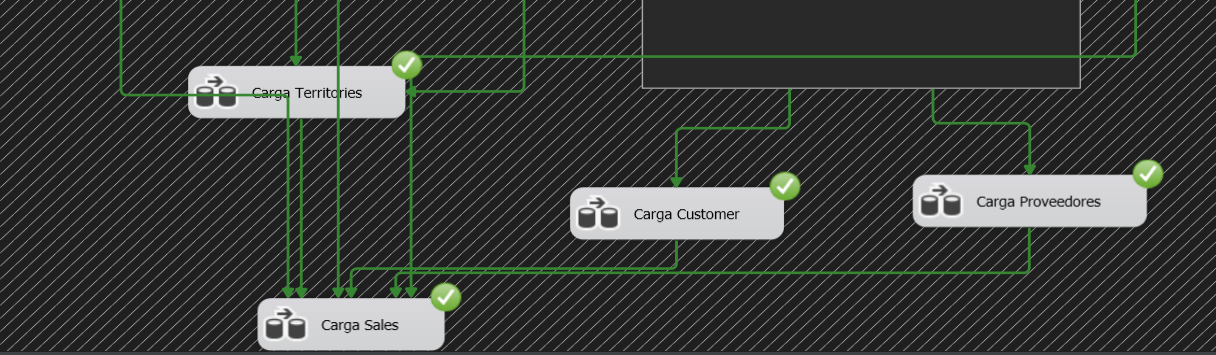
\includegraphics[width=1\textwidth]{image/flujo_north_3.png}
		\caption{Flujo ETL Nortwind PT3}
		\label{fig:7}
	\end{figure}
	
	
	\begin{figure}[H]
		\centering
		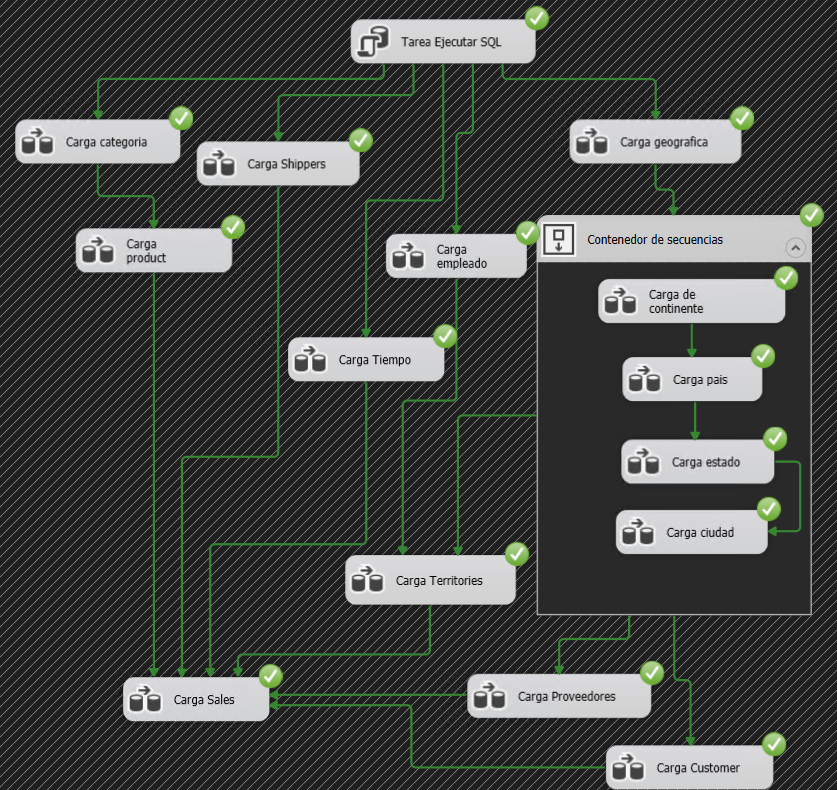
\includegraphics[width=1\textwidth]{image/flujo_north_completo.png}
		\caption{Flujo ETL Nortwind completo}
		\label{fig:8}
	\end{figure}
	

	
	\subsection{Dificultades en Northwind}
	
	Debido a que el archivo original, Time.xls, estaba en un formato antiguo, fue necesario transformarlo a Time.xlsx. Aunque se intentó especificar el origen como "Excel 1997", no fue posible reconocer la columna correctamente. Tras realizar la conversión al formato Excel 2007-2010, el sistema logró identificar sin problemas la columna Feuil.
	
	Otra dificultad que enfrentamos fue durante el vaciado del almacén de datos, específicamente con las claves foráneas (FK). El problema surgía porque, en algunos casos, se eliminaban primero los registros asociados a la clave primaria (PK), lo que generaba conflictos con las claves foráneas dependientes. Para resolver este inconveniente, decidimos deshabilitar temporalmente las restricciones de las claves foráneas antes de realizar el vaciado del almacén y, una vez completado, las volvimos a habilitar.
	
	-- Desactivar las restricciones de clave foránea temporalmente
	EXEC sp\_MSForEachTable 'ALTER TABLE ? NOCHECK CONSTRAINT ALL';
	
	-- Reactivar las restricciones de clave foránea
	EXEC sp\_MSForEachTable 'ALTER TABLE ? WITH CHECK CHECK CONSTRAINT ALL';
	
	
	\section{ETL del almacén de datos de pacientes con patologías respiratorias}
	
	\textbf{Aquí creo que sería bueno aclarar lo de las claves del hecho y sobre porque se guardo el atributo PatientOG}
	Antes de realizar el proceso ETL, es necesario dejar claras algunas decisiones tomadas en el llenado del \textbf{Data Warehouse (DW)}, específicamente en relación con el hecho. Según la teoría, las claves foráneas de un hecho deben ser las claves primarias de las tablas relacionadas. Sin embargo, en nuestro caso, hemos optado por una solución que permite evitar trabajo extra al llenar las tablas intermedias, sin perder información. En lugar de utilizar tres claves foráneas diferentes, hemos creado una clave autogenerada como clave primaria (PK) que sea única para cada combinación de \texttt{TiempoID}, \texttt{HospitalID} y \texttt{UniquePID}. De esta forma, mantenemos la eficacia de acceder a las claves foráneas \texttt{TiempoID}, \texttt{HospitalID} y \texttt{UniquePID} desde otras tablas, pero sin la necesidad de escribir tres claves diferentes.
	
	Otra decisión importante fue almacenar ciertas claves antiguas en algunas tablas para facilitar la herencia de claves foráneas. Por ejemplo, en el hecho hemos almacenado la clave antigua del paciente, \texttt{patientUnitStayID\_og}, con el objetivo de facilitar la herencia de la clave primaria del hecho \texttt{IngresoUCI}.
	
	El resto de claves en las tablas serán autogeneradas. Un ejemplo de esto es el siguiente código para la tabla \texttt{Ethnicity}:
	
	\begin{verbatim} ALTER TABLE Ethnicity ADD ethnicityID INT IDENTITY(1,1) PRIMARY KEY; 
	\end{verbatim}
	
	
	Así mismo en este apartado se explicará más detenidamente todo el proceso de carga aplicado para este proyecto, partiendo desde el uso de \textit{Microsoft SQL Server Management Studio} para restaurar las bases de datos, tanto la fuente de datos correspondiente a La base de datos de investigación colaborativa, \textit{eICU Collaborative Research Database}, disponible en este \href{https://uma365-my.sharepoint.com/:u:/g/personal/rmluque_uma_es/EebuEtDjp8VImt-_PhweiZMBu1_7XkPqZHkD74iGgg0fXQ?e=lOivcI}{enlace}. Además del \textit{DDL} creado específicamente para esta actividad, accesible en el repositorio de GitHub a través de este \href{https://github.com/Diegodepab/almacen_UCI_Sanitaria/blob/main/ETL/base_de_datos.ddl}{enlace}. A partir de un enfoque para pacientes con patología respiratorias 
	
	Una vez restaurada las bases de datos y preparadas sus conexiones para el repositorio de \textit{Visual Studio, SQL Server Integration Services Project}, se podrá empezar el proceso de ETL a nuestro nuevo Data Warehouse (DW), como se observa en la figura \ref{fig:2} al contar con gran cantidad de tablas en el modelo copo de nieve resultará bastantes flujos de datos en nuestro repositorio.
	
	
	\begin{figure}[H]
		\centering
		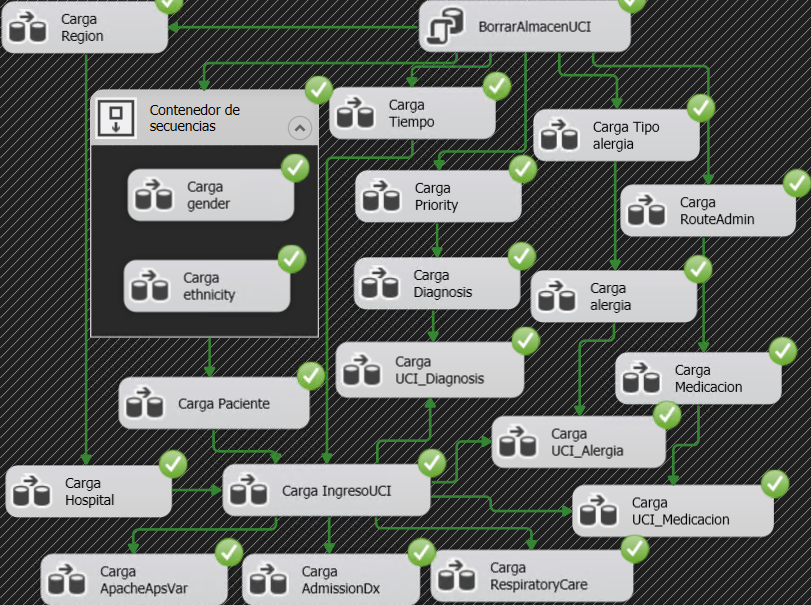
\includegraphics[width=1\textwidth]{image/100_ETL_ejecutandose.png}
		\caption{Flujo de control una vez acabado el ETL}
		\label{fig:2}
	\end{figure}
	
	A continuación la explicación tarea por tarea de cada actividad planteada en el flujo de control, es importante destacar que el trabajo sigue cierta secuencialidad en algunas secciones que dependen de fases anteriores, se íntentará destacar la paralelización de tareas y la tarea previa a cada actividad pero es importante seguir las flechas mostradas en la figura \ref{fig:2}. 
	
	La primera actividad por excelencia en cualquier proyecto de integración de servicios es \textbf{BorrarAlmacenUCI}, para evitar duplicar datos al crear la carga de datos, como se observa en la figura \ref{fig:3} se aplica una \textit{Tarea Ejecutar SQL}, indicando el \textit{SQLStatment y IsQueryStoredProcedure}, para este punto se debe volver a \textit{SQL Server Management} para crear un procedimiento almacenado (en la database, la carpeta \textit{Programmability y StoredProcedures}), el cual se encargará de deshabilitar las restricciones de claves foráneas (útil para esta ocasión donde se desea eliminar todas las tablas para preparar el ETL y evitar errores por borrar tablas en un orden equivocado) se elimina los registros de cada tabla y por último habilita nuevamente las restricciones de claves foráneas, a través de este \href{https://github.com/Diegodepab/almacen_UCI_Sanitaria/blob/main/ETL/BorrarAlmacenUCI.sql}{enlace podrá ver el código detalladamente}.

	\begin{figure}[H]
		\centering
		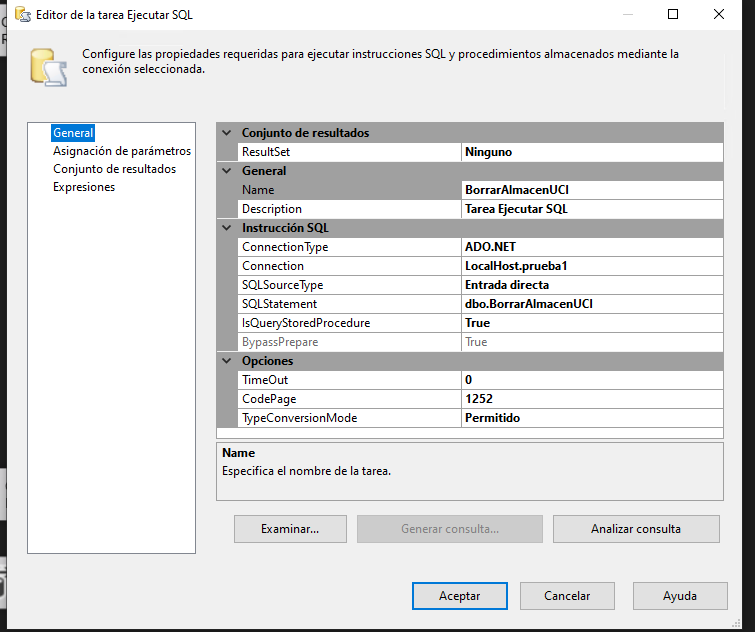
\includegraphics[width=1\textwidth]{image/101_BorrarAlmacenUCI.png}
		\caption{Ventana de información de BorrarAlmacenUCI, ya configurada}
		\label{fig:3}
	\end{figure}
	
	Una vez realizado el borrado de las cargas anteriores, se puede proceder con las tareas reales de carga del almacén. Es fundamental evitar la secuencialidad en el trabajo, por lo que los flujos de datos que puedan ejecutarse en paralelo deben iniciarse. Tras ejecutar el proceso \textit{BorrarAlmacenUCI}, se inician inmediatamente los siguientes seis flujos de datos:
	
	
	\subsection{Carga de Región}
	
	En el caso de \textbf{Carga Region} se puede las tareas que se realizan en el flujo de datos en la figura \ref{fig:4}, en esta misma 
	
	\begin{figure}[H]
		\centering
		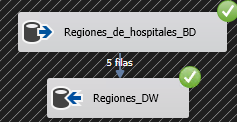
\includegraphics[width=0.35\textwidth]{image/103_region.png}
		\caption{Carga de las distintas regiones para los hospitales de la base de datos elCU}
		\label{fig:4}
	\end{figure}
	
	
	\subsection{Carga de Género y Etnia}
	
	Utilizamos un contenedor de secuencias. Se lleva a cabo debido a que género y etnia son jerarquías paralelas y consideramos correcto establecer un orden en sus cargas.
	
	Para la \textbf{carga de género} (ver Figura \ref{fig:10}), se utilizó como origen la base de datos \textbf{[eICU Collaborative Research Database]}. En lugar de emplear directamente la tabla de género, se utilizó la siguiente consulta:
	
	\begin{verbatim} SELECT DISTINCT Gender FROM Patient \end{verbatim}
	
	El objetivo de esta consulta fue almacenar únicamente los géneros distintos, incluyendo los valores \textbf{NULL} para evitar discriminar a pacientes cuyo género no fue registrado.
	
	Adicionalmente, se realizó una conversión de datos, ya que en el almacén de destino el campo \texttt{genderString} está definido como una cadena Unicode (\texttt{DT\_WSTR}) con una longitud de 25 caracteres. Finalmente, se almacenaron los géneros distintos en el destino, y la clave \texttt{genderID} fue autogenerada en la nueva base de datos.
	
	\begin{figure}[H]
		\centering
		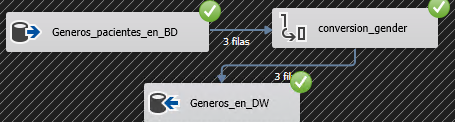
\includegraphics[width=1\textwidth]{image/106_carga_generos.png}
		\caption{Carga géneros}
		\label{fig:10}
	\end{figure}
	
	En la \textbf{carga de etnia} se siguió la misma lógica utilizada para la carga de géneros. Se realizó una conversión de datos para ajustar el campo \texttt{Ethnicity} del origen al campo \texttt{ethnicityString} del destino. Finalmente, los valores procesados se almacenaron en la nueva base de datos.
	
	\begin{figure}[H]
		\centering
		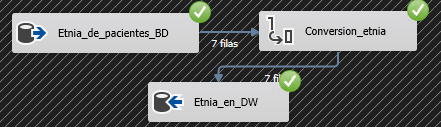
\includegraphics[width=1\textwidth]{image/107_carga_etnia.png}
		\caption{Carga etnia}
		\label{fig:11}
	\end{figure}
	
	
	\subsection{Carga Tiempo}
	
	Para la \textbf{carga de la tabla tiempo \ref{fig:18}}, únicamente se trasladaron las tuplas de la tabla \texttt{Paciente} de la base de datos del eICU, específicamente los campos \texttt{HospitalDischargeTime24} y \texttt{HospitalDischargeYear}. El campo \texttt{TiempoID}, que se encuentra en el destino, fue autogenerado automáticamente al realizar el almacenamiento de los datos.
	
	\begin{figure}[H]
		\centering
		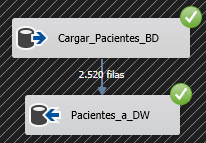
\includegraphics[width=1\textwidth]{image/109_carga_tiempo.png}
		\caption{Carga Tiempo}
		\label{fig:18}
	\end{figure}
	
	\subsection{Carga Priority}
	
	Para la \textbf{carga de prioridad} se siguió exactamente el mismo procedimiento utilizado para género y etnia. Se seleccionaron únicamente las distintas prioridades asociadas a los diagnósticos mediante la siguiente consulta:
	
	\begin{verbatim} SELECT DISTINCT DiagnosisPriority FROM Diagnosis \end{verbatim}
	
	Posteriormente, los valores obtenidos se insertaron en el \textbf{Data Warehouse (DW)}.
	
	\begin{figure}[H]
		\centering
		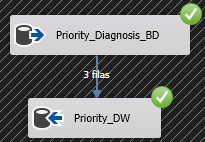
\includegraphics[width=1\textwidth]{image/111_carga_priority.png}
		\caption{Carga Priority}
		\label{fig:20}
	\end{figure}
	
	\subsection{Carga Tipo}
	
	\subsection{Carga RouteAdmin}
	
	\subsection{Carga Hospital}
	
	Para la \textbf{carga de hospital}, se utilizó como origen la tabla \texttt{Hospital} de la base de datos \textbf{eICU}. Posteriormente, se realizó una conversión del atributo \texttt{Region} de la tabla \texttt{Hospital}, transformándolo a una cadena (\texttt{DT\_STR}) con una longitud de 64 caracteres. 
	
	\begin{figure}[H]
		\centering
		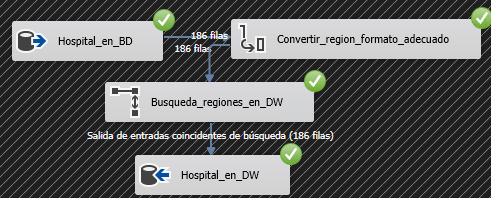
\includegraphics[width=1\textwidth]{image/105_cargahospital.png}
		\caption{Carga Hospital}
		\label{fig:16}
	\end{figure}
	
	Esta transformación fue necesaria para realizar un \textit{join} mediante un elemento \textit{lookup} de \textbf{SQL Integration Services}, cuyo objetivo fue buscar las tuplas que coincidieran en región y, a partir de ahí, obtener el correspondiente \texttt{regionID} \ref{fig:22}.
	
	\begin{figure}[H]
		\centering
		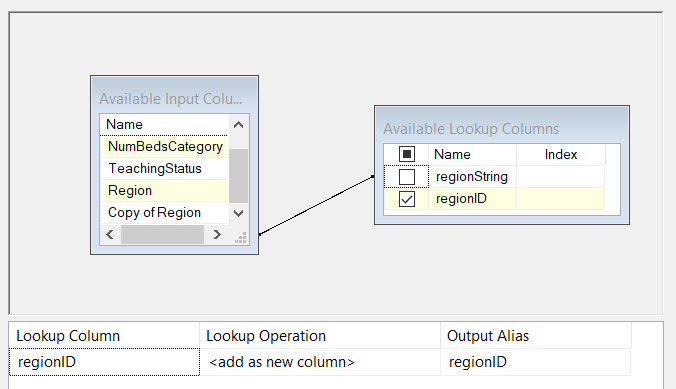
\includegraphics[width=1\textwidth]{image/105_cargahospital_lookup.png}
		\caption{Busqueda\_regiones\_en\_DW}
		\label{fig:22}
	\end{figure}

	
	Finalmente, se almacenaron los siguientes campos en el destino\ref{fig:23}:
	
	\begin{itemize}
		\item \texttt{HospitalID} del \textbf{eICU}, renombrado como \texttt{hospitalID\_og}, para permitir que \texttt{IngresoUCI} herede la nueva clave \texttt{HospitalID} generada en nuestro \textbf{DW}.
		\item \texttt{regionID}, como clave foránea heredada de la tabla \texttt{Region}.
	\end{itemize}
	
	\begin{figure}[H]
		\centering
		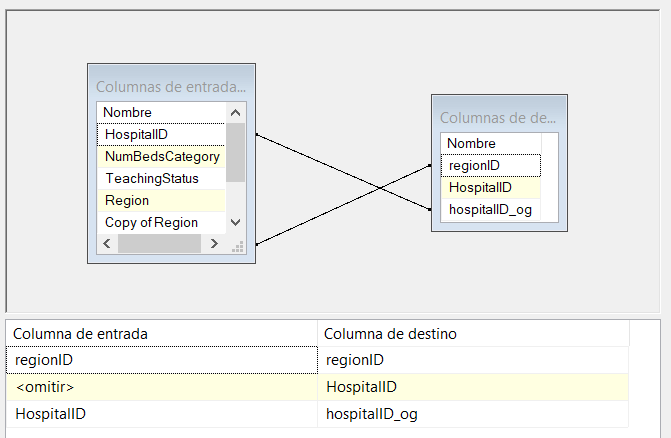
\includegraphics[width=1\textwidth]{image/105_cargahospital_destino.png}
		\caption{Hospital\_en\_DW}
		\label{fig:23}
	\end{figure}

	
	\subsection{Carga Paciente}
	
	\begin{figure}[H]
		\centering
		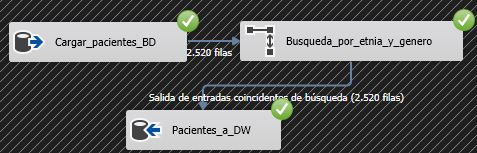
\includegraphics[width=1\textwidth]{image/108_carga_paciente.png}
		\caption{Carga Paciente}
		\label{fig:17}
	\end{figure}
	
	Para la \textbf{carga de paciente}, se utilizó como origen la tabla \texttt{Patient} de la base de datos \textbf{eICU}. En este proceso, se seleccionaron los atributos especificados en la Figura \ref{fig:24}.
	
	
	\begin{figure}[H]
		\centering
		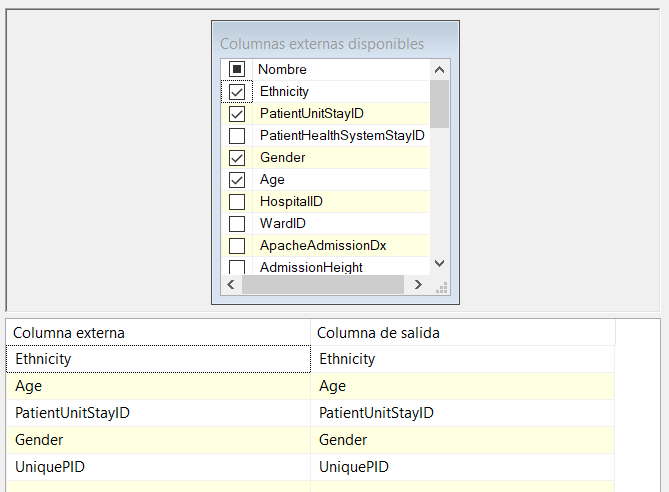
\includegraphics[width=1\textwidth]{image/108_carga_paciente_origen.png}
		\caption{Origen del flujo}
		\label{fig:24}
	\end{figure}
	
	Posteriormente, se realizará un \textit{lookup} para efectuar un \textit{join} entre los campos \texttt{Ethnicity} y \texttt{Gender} de la base de datos \textbf{eICU}, y los campos \texttt{ethnicityString} y \texttt{genderString} obtenidos a partir de la siguiente consulta sobre nuestro \textbf{DW}(ver Figura \ref{fig:25}):
	
	\begin{verbatim}
		SELECT * FROM Ethnicity, Gender
	\end{verbatim}
	
	
	\begin{figure}[H]
		\centering
		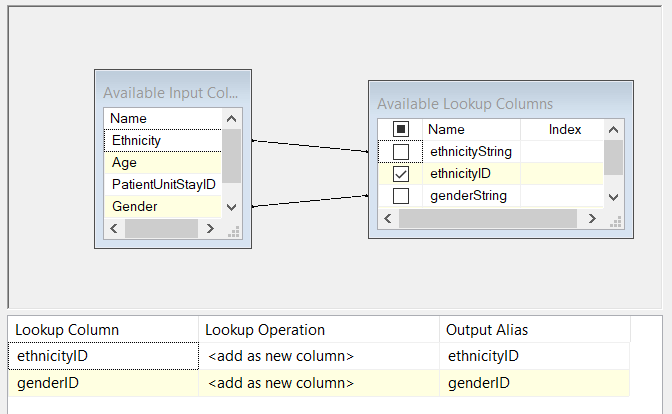
\includegraphics[width=1\textwidth]{image/108_carga_paciente_lookup.png}
		\caption{Busqueda\_por\_etnia\_y\_genero}
		\label{fig:25}
	\end{figure}

	
	Por último, se insertarán los siguientes atributos en el destino (ver Figura \ref{fig:27}):
	
	\begin{figure}[H]
		\centering
		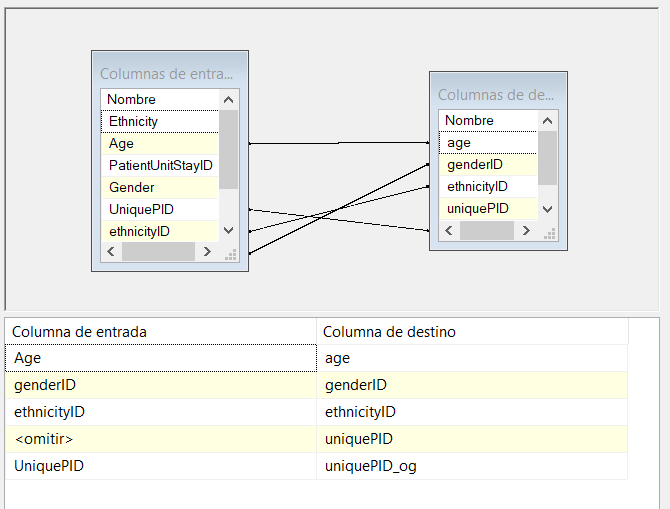
\includegraphics[width=0.8\textwidth]{image/108_carga_paciente_destino.png}
		\caption{Pacientes\_a\_DW}
		\label{fig:27}
	\end{figure}

	
	Además, se incluirá el atributo \texttt{UniquePID}, ya que es necesario para permitir que \texttt{IngresoUCI} herede la clave foránea (\texttt{FK}) de \texttt{Paciente}.
	
	\subsection{Carga IngresoUCI}
	
	\begin{figure}[H]
		\centering
		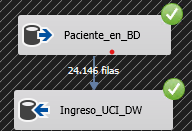
\includegraphics[width=1\textwidth]{image/110_carga_ingreso.png}
		\caption{Carga IngresoUCI}
		\label{fig:19}
	\end{figure}
	
	Para la carga de \texttt{IngresoUCI}, se utilizó como origen la siguiente consulta, mostrada en la Figura \ref{fig:26}:
	
	\begin{figure}[H]
		\centering
		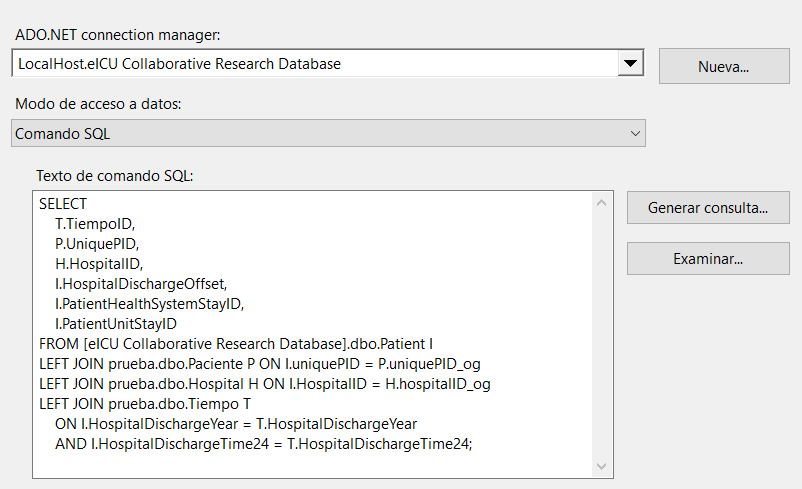
\includegraphics[width=0.8\textwidth]{image/110_carga_ingreso_origen.png}
		\caption{Paciente\_en\_BD}
		\label{fig:26}
	\end{figure}
	
	\textbf{Nota:} Cuando se menciona \texttt{prueba.dbo}, nos referimos a nuestra nueva base de datos/DW, ya que así la hemos denominado.
	
	La consulta selecciona varios atributos de la base de datos \textbf{eICU Collaborative Research Database} y los combina con datos de nuestro \textbf{Data Warehouse (DW)}, específicamente de las tablas \texttt{Paciente}, \texttt{Hospital}, y \texttt{Tiempo}, utilizando \textit{joins} (uniones).
	
	\textbf{Descripción de la consulta:}
	
	\begin{itemize} \item \textbf{Campos seleccionados:} 
		\begin{itemize} 
			\item \texttt{TiempoID}: Proviene de la tabla \texttt{Tiempo}, representando el identificador del tiempo del paciente. \item \texttt{UniquePID}: Es el identificador único del paciente, que se obtiene de la tabla \texttt{Paciente}. \item \texttt{HospitalID}: Representa el identificador del hospital, proveniente de la tabla \texttt{Hospital}. \item \texttt{HospitalDischargeOffset}: Muestra el tiempo que ha pasado desde que el paciente fue dado de alta del hospital. \item \texttt{PatientHealthSystemStayID}: Identificador de la estancia del paciente en el sistema de salud. \item \texttt{PatientUnitStayID}: Identificador de la unidad en la que el paciente estuvo durante su estancia. 
		\end{itemize}
		
		\item \textbf{Proceso de unión (joins):}
		La consulta usa \textbf{LEFT JOIN} para combinar las tablas, lo que significa que se toman todos los registros de la tabla de la izquierda (de la base de datos \texttt{eICU}) y los registros coincidentes de las tablas de la derecha (de nuestro DW). Si no hay coincidencia, los valores de las tablas del DW serán \texttt{NULL}.
		
		\begin{itemize}
			\item \textbf{Primer JOIN:} Se une la tabla \texttt{Patient} de \texttt{eICU} (aliased como \texttt{I}) con la tabla \texttt{Paciente} de nuestro DW (aliased como \texttt{P}), usando el campo \texttt{uniquePID} de ambas tablas. Aquí, se mapea el \texttt{uniquePID} de \texttt{eICU} al campo \texttt{uniquePID\_og} de \texttt{Paciente} en el DW.
			
			\item \textbf{Segundo JOIN:} Se une la tabla \texttt{Patient} de \texttt{eICU} con la tabla \texttt{Hospital} en nuestro DW (aliased como \texttt{H}), usando el campo \texttt{HospitalID}. Se compara \texttt{HospitalID} de \texttt{eICU} con \texttt{hospitalID\_og} en \texttt{Hospital} en el DW.
			
			\item \textbf{Tercer JOIN:} Se une la tabla \texttt{Patient} de \texttt{eICU} con la tabla \texttt{Tiempo} en el DW (aliased como \texttt{T}), utilizando los campos \texttt{HospitalDischargeYear} y \texttt{HospitalDischargeTime24} de \texttt{eICU} y comparándolos con los mismos campos en la tabla \texttt{Tiempo} de nuestro DW.
		\end{itemize}
		
		\item \textbf{Resultado final:} La consulta extrae los datos de \texttt{eICU} y los enlaza con la información relevante de nuestro DW, lo que permite que los registros en la tabla \texttt{IngresoUCI} contengan las claves correctas de las tablas de nuestro DW (como \texttt{Paciente}, \texttt{Hospital}, y \texttt{Tiempo}).
	\end{itemize}
	
	Por último, se insertaron los datos en IngresoUCI de nuestro DW:
	
	\begin{figure}[H]
		\centering
		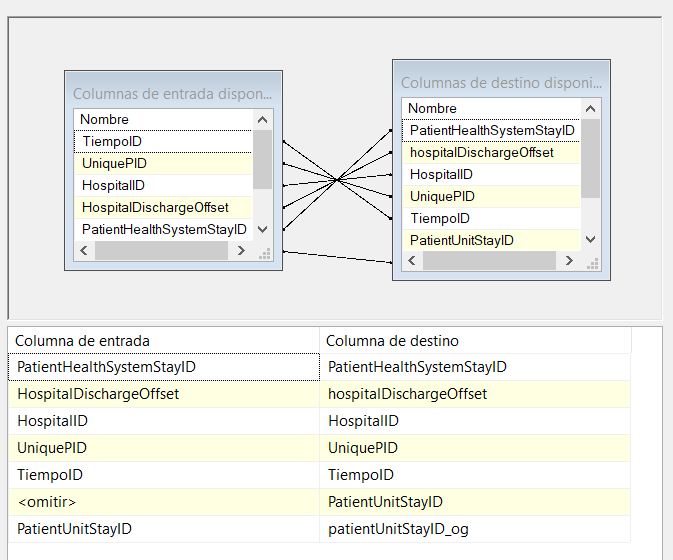
\includegraphics[width=1\textwidth]{image/110_carga_ingreso_destino.png}
		\caption{Ingreso\_UCI\_DW}
		\label{fig:28}
	\end{figure}
	
	\subsection{Carga Diagnosis}
	
	\begin{figure}[H]
		\centering
		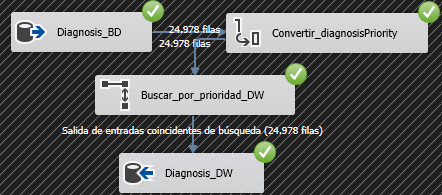
\includegraphics[width=1\textwidth]{image/112_carga_diagnosis.png}
		\caption{Carga Diagnosis}
		\label{fig:21}
	\end{figure}
	
	Para la carga de \texttt{Diagnosis}, se tomó como origen la tabla \texttt{Diagnosis} del \textbf{eICU}. Posteriormente, se realizó una conversión del atributo \texttt{DiagnosisPriority} a tipo cadena \texttt{[DT\_STR]} con longitud 10.
	
	A continuación, se realizará un \textit{join} entre \texttt{Copy of DiagnosisPriority} y \texttt{priorityString} de la tabla \texttt{Priority} de nuestra base de datos/DW, y se seleccionará el \texttt{priorityID} para que pueda ser heredado por \texttt{Diagnosis} en nuestro \textbf{DW} (ver Figura \ref{fig:29}).
	
	\begin{figure}[H]
		\centering
		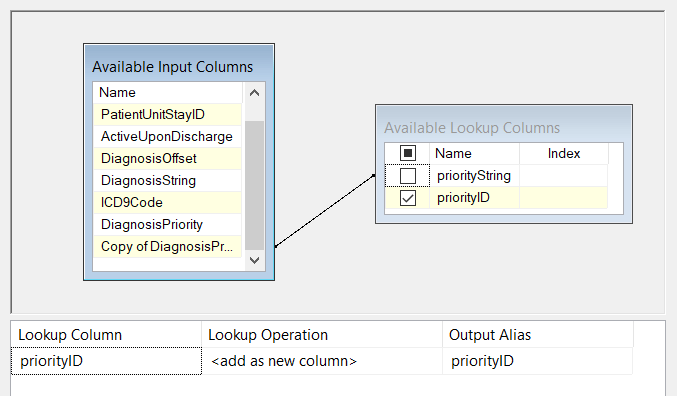
\includegraphics[width=1\textwidth]{image/112_carga_diagnosis_lookup.png}
		\caption{Buscar\_por\_prioridad\_DW}
		\label{fig:29}
	\end{figure}
	
	Estos serán los atributos de \texttt{Diagnosis} en nuestro \textbf{DW}:
	
	\begin{figure}[H]
		\centering
		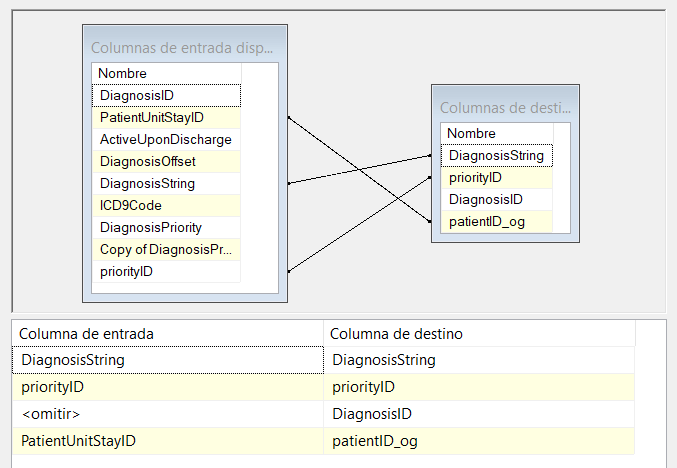
\includegraphics[width=0.8\textwidth]{image/112_carga_diagnosis_destino.png}
		\caption{Diagnosis\_DW}
		\label{fig:30}
	\end{figure}

	% Sections
	\section{Dificultades encontradas}
	
	
	Una de las principales dificultades fue la complejidad de la base de datos eICU, que incluye una gran cantidad de tablas y atributos. Esto exigió un análisis detallado para identificar las tablas y campos clave en un modelo centrado en pacientes con enfermedades respiratorias. Además, enfrentamos problemas de permisos al intentar visualizar el modelo relacional en SQL Server, lo que requirió modificar las autorizaciones del propietario de la base de datos para acceder a los diagramas de relación.
	
	Además el comienzo del trabajo podría ser lo más angustioso, al tener tanta información y opciones llega a ser un poco abrumador, desde la selección de una población concreta y modelar un almacén para dicha población termina dejando muchas dudas sobre cuantas tablas es esperable eliminar, si se esta simplificando de más o se esta tomando una decisión que afectará los siguientes apartados. 
	
	\section{Conclusiones}
	
	


	\section{Github y conjunto de instrucciones para su correcto despliegue en SQL Server.}

	Todo el proyecto está accesible en github \cite{depab2024} donde se detalla más específicamente como desplegar en SQL.
	%%%%%%%%%%%%%%%%%%%%%%%%%%%%%%%%%%%%%%%%%%%%%%%%%%%%%%%%%%%%%%%%%%%%%%%%%%%
	\printbibliography
	
	
	%% Back Cover
	
\includepdf[noautoscale=true, width=\paperwidth]{backcover.pdf}
	
\end{document}